% No new page; first page call under this section. see ProjectStructureSrc . 
\visHeader

Now\hypertarget{projectStructure vis}{} that everything is installed and setup properly, let's take a closer look at the different workspaces and our workflow.
Before we continue, please make a few slight adjustments to EA so you can easily compare your current workspace to our screenshots:
\begin{itemize}

\item[$\blacktriangleright$] Select ``Tools/Options/Standard Colors'' in EA, and set your colours to reflect Fig.~\ref{fig_standardColoursEA}.
This is advisable but you are, of course, free to choose your own colour schema.

\begin{figure}[htbp]
  \centering
  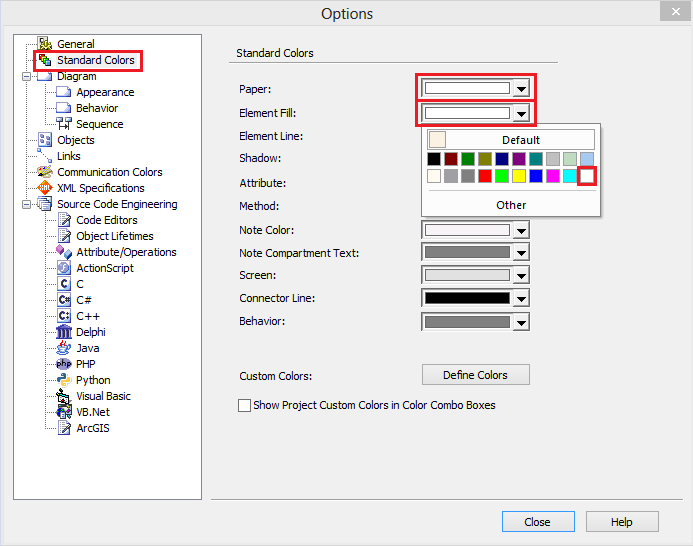
\includegraphics[width=0.8\textwidth]{standardColours}
  \caption{Our choice of standard colours for diagrams in EA.}
  \label{fig_standardColoursEA}
\end{figure}

\item[$\blacktriangleright$] In the same dialogue, select ``Diagram/Appearance'' and reflect the settings in Fig.~\ref{fig_standardAppearanceEA}.
Again, this is just a suggestion and not mandatory.

\item[$\blacktriangleright$] Last but not least, and still in the same dialogue, select ``Source Code Engineering'' and be sure to choose ``Ecore'' as the default language for code generation (Fig.~\ref{fig_standardSCEEA}). This setting \emph{is} mandatory, and very important.
\end{itemize}

In your EA ``workspace'' (actually referred to as an \emph{EA project}\footnote{Words are set in italics when they represent concepts that are introduced or defined  in the corresponding paragraph for the first time.}) take a careful  look at the project structure:  The root node \texttt{Demo}\footnote{Words set  in a \texttt{mono-space font} refer to things that you should find in a tool,  dialogue, figure or code.} is called a \emph{model}

%%

\begin{figure}[htbp]
  \centering
  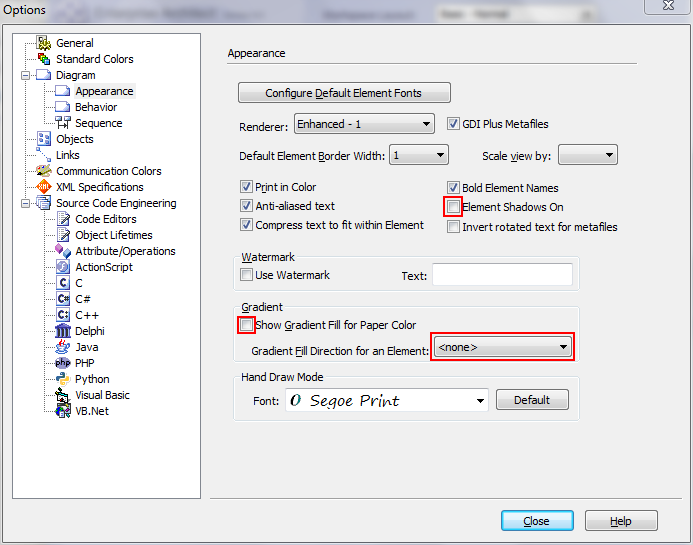
\includegraphics[width=0.8\textwidth]{standardAppearance}
  \caption{Our choice of the standard appearance for model elements.}
  \label{fig_standardAppearanceEA}
\end{figure}

\begin{figure}[htbp]
    \centering
    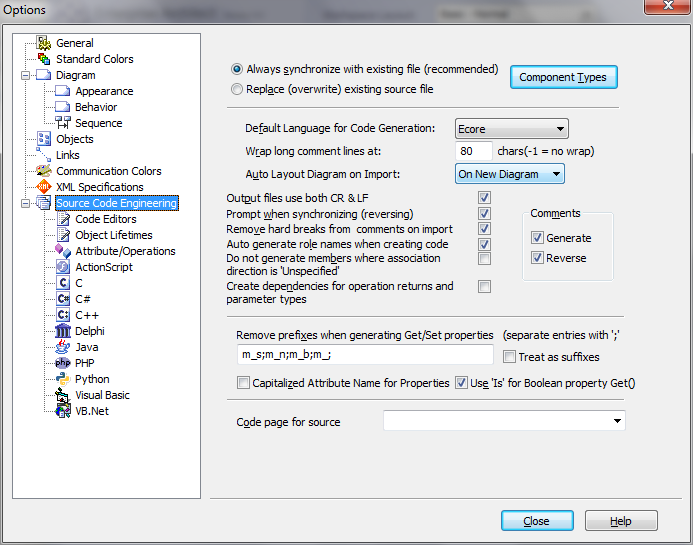
\includegraphics[width=0.8\textwidth]{standardCodeEngineering}
    \caption{Make sure you set the standard language to Ecore.}
    \label{fig_standardSCEEA}
 \end{figure}

in EA lingo, and is used as a  container to group a set of related \emph{packages}. 
In our case, \texttt{Demo}  consists of a single package \texttt{DoubleLinkedListLanguage}.
An EA project however, can consist of numerous models that in turn, group numerous packages.

Now switch to your \emph{Eclipse workspace} and note the two nodes named \texttt{Spe\-ci\-fi\-ca\-tions} and \texttt{Demo}.  These nodes, used to group related \emph{Eclipse projects} in an Eclipse workspace, are called \emph{working sets}. % (funny?): Remember how I said we'd explain the nodes in a moment 2 pages ago? That moment is now.
The working set \texttt{Spe\-ci\-fi\-ca\-tions} contains all \emph{metamodel projects} in a  workspace. A metamodel project contains a single EAP (EA project) file and is used to communicate with EA and initiate code generation by simply pressing F5 or choosing ``refresh'' from the context menu.
In our case, \texttt{Specifications} should contain a single metamodel project \texttt{Demo} containing our EA project file  \texttt{Demo.eap}.
% \% end common
 
Figure~\ref{fig_fromEAtoEclipse} depicts how the Eclipse working set \texttt{Demo} and its contents were generated from the EA model \texttt{Demo}.
Every model in EA is mapped to a working set in Eclipse with the same name. 
From every package in the EA model, an Eclipse project is generated, also with the same name. These projects, however, are of a different \emph{nature} than for example metamodel projects or normal Java projects, and are called \emph{repository projects}.  
A nature is Eclipse lingo for ``project type'' and is visually indicated by a corresponding nature icon on the project folder.
Our  metamodel projects sport a spanking little class diagram symbol. 
Repository projects are generated automatically
%%
with a certain project structure according to our conventions.  
The  \texttt{model} subfolder is probably most important, and contains an  \emph{Ecore model}.  
Ecore is a metamodelling language that provides building  blocks like \emph{classes} and \emph{references} for defining the  static structure (concepts and relations between concepts) of a system.  

The  export function of our EA plugin generates a valid Ecore model from the  corresponding EA model and persists it as an XML file in the \texttt{model}  subfolder.  
In our concrete example, this is the \texttt{DoubleLinkedListLanguage.ecore} file.  
Go ahead and double-click it to open the file in a simple tree-view editor in Eclipse.  
If you are really interested in the nitty-gritty details or have a masochistic hang, right-click the file and select ``Open With/Text Editor''.

Figure~\ref{fig_fromEAtoEclipse} also depicts how the class \texttt{Node} in the EA model is mapped to the Java interface \texttt{Node}.  
Double-click \texttt{Node.java} and take a look at the methods declared in the interface.
These correspond directly to the methods declared in the modelled \texttt{Node} class.  
Indicated by the source folders \texttt{src}, \texttt{injection} and \texttt{gen}, we advocate a clean separation of hand-written (this should go in \texttt{src} and \texttt{injection}) and generated code (lands automatically in \texttt{gen}).  
As we shall see later in the handbook, hand-written code can be integrated in generated classes vio Injections. 
This is sometimes more elegant for small helper functions or necessary for String manipulation for instance.

%%

\begin{figure}[htbp]
    \centering
  \includegraphics[width=\textwidth]{bothexplorers}
    \caption{From EA to Eclipse}
    \label{fig_fromEAtoEclipse}
\end{figure}

Have you noticed the methods of the \texttt{Node} class in our EA model? 
Now hold on tight -- each method can be \emph{modelled} completely in EA and the corresponding implementation in Java is generated automatically and placed in \texttt{NodeImpl}.  
Just in case you didn't get it: The behavioural or dynamic aspects of a system can be completely modelled in an abstract, platform (programming language) independent fashion using a blend of activity  diagrams and a ``graph pattern'' language called \textit{Story Driven Modelling} (SDM).  
In our EA project, these ``Stories'', ``Story Models'' or simply ``SDMs'' are  placed in SDM Containers named according to the method they implement.  
E.g.  \texttt{$\guillemotleft$SDM Container$\guillemotright$ insertNodeAfter SDM} for the method  \texttt{insertNodeAfter(Node)} as depicted in
Fig.~\ref{fig_fromEAtoEclipse}.  
We'll dedicate an entire handbook understanding why SDMs are so  {\huge crazily} cool!
 
To recap all we've discussed, let's consider the complete workflow as depicted in Figure~\ref{fig_Overview}. 
We started with a concise model in EA, simple and independent of any platform specific details~(1).  
Our EA model consists not only of static aspects modelled as a class diagram~(2), but also of dynamic
aspects modelled using SDM~(3).  After exporting the model and code generation~(4), we basically switch from \emph{modelling} to \emph{programming} in a specific general purpose programming language (Java).  
On this lower \emph{level of abstraction}, we can flesh out the generated repository~(5) if necessary, and mix as appropriate with hand-written code and libraries.  Our abstract specification of behaviour (methods) in SDM is translated to a series of method calls that form the body of the corresponding Java method~(6).

%%
\pagebreak
\fancyfoot[R]{  $\triangleright$ \hyperlink{codeGen common}{Next task} }

\vspace*{3cm}

\begin{figure}[htbp]
	\centering
  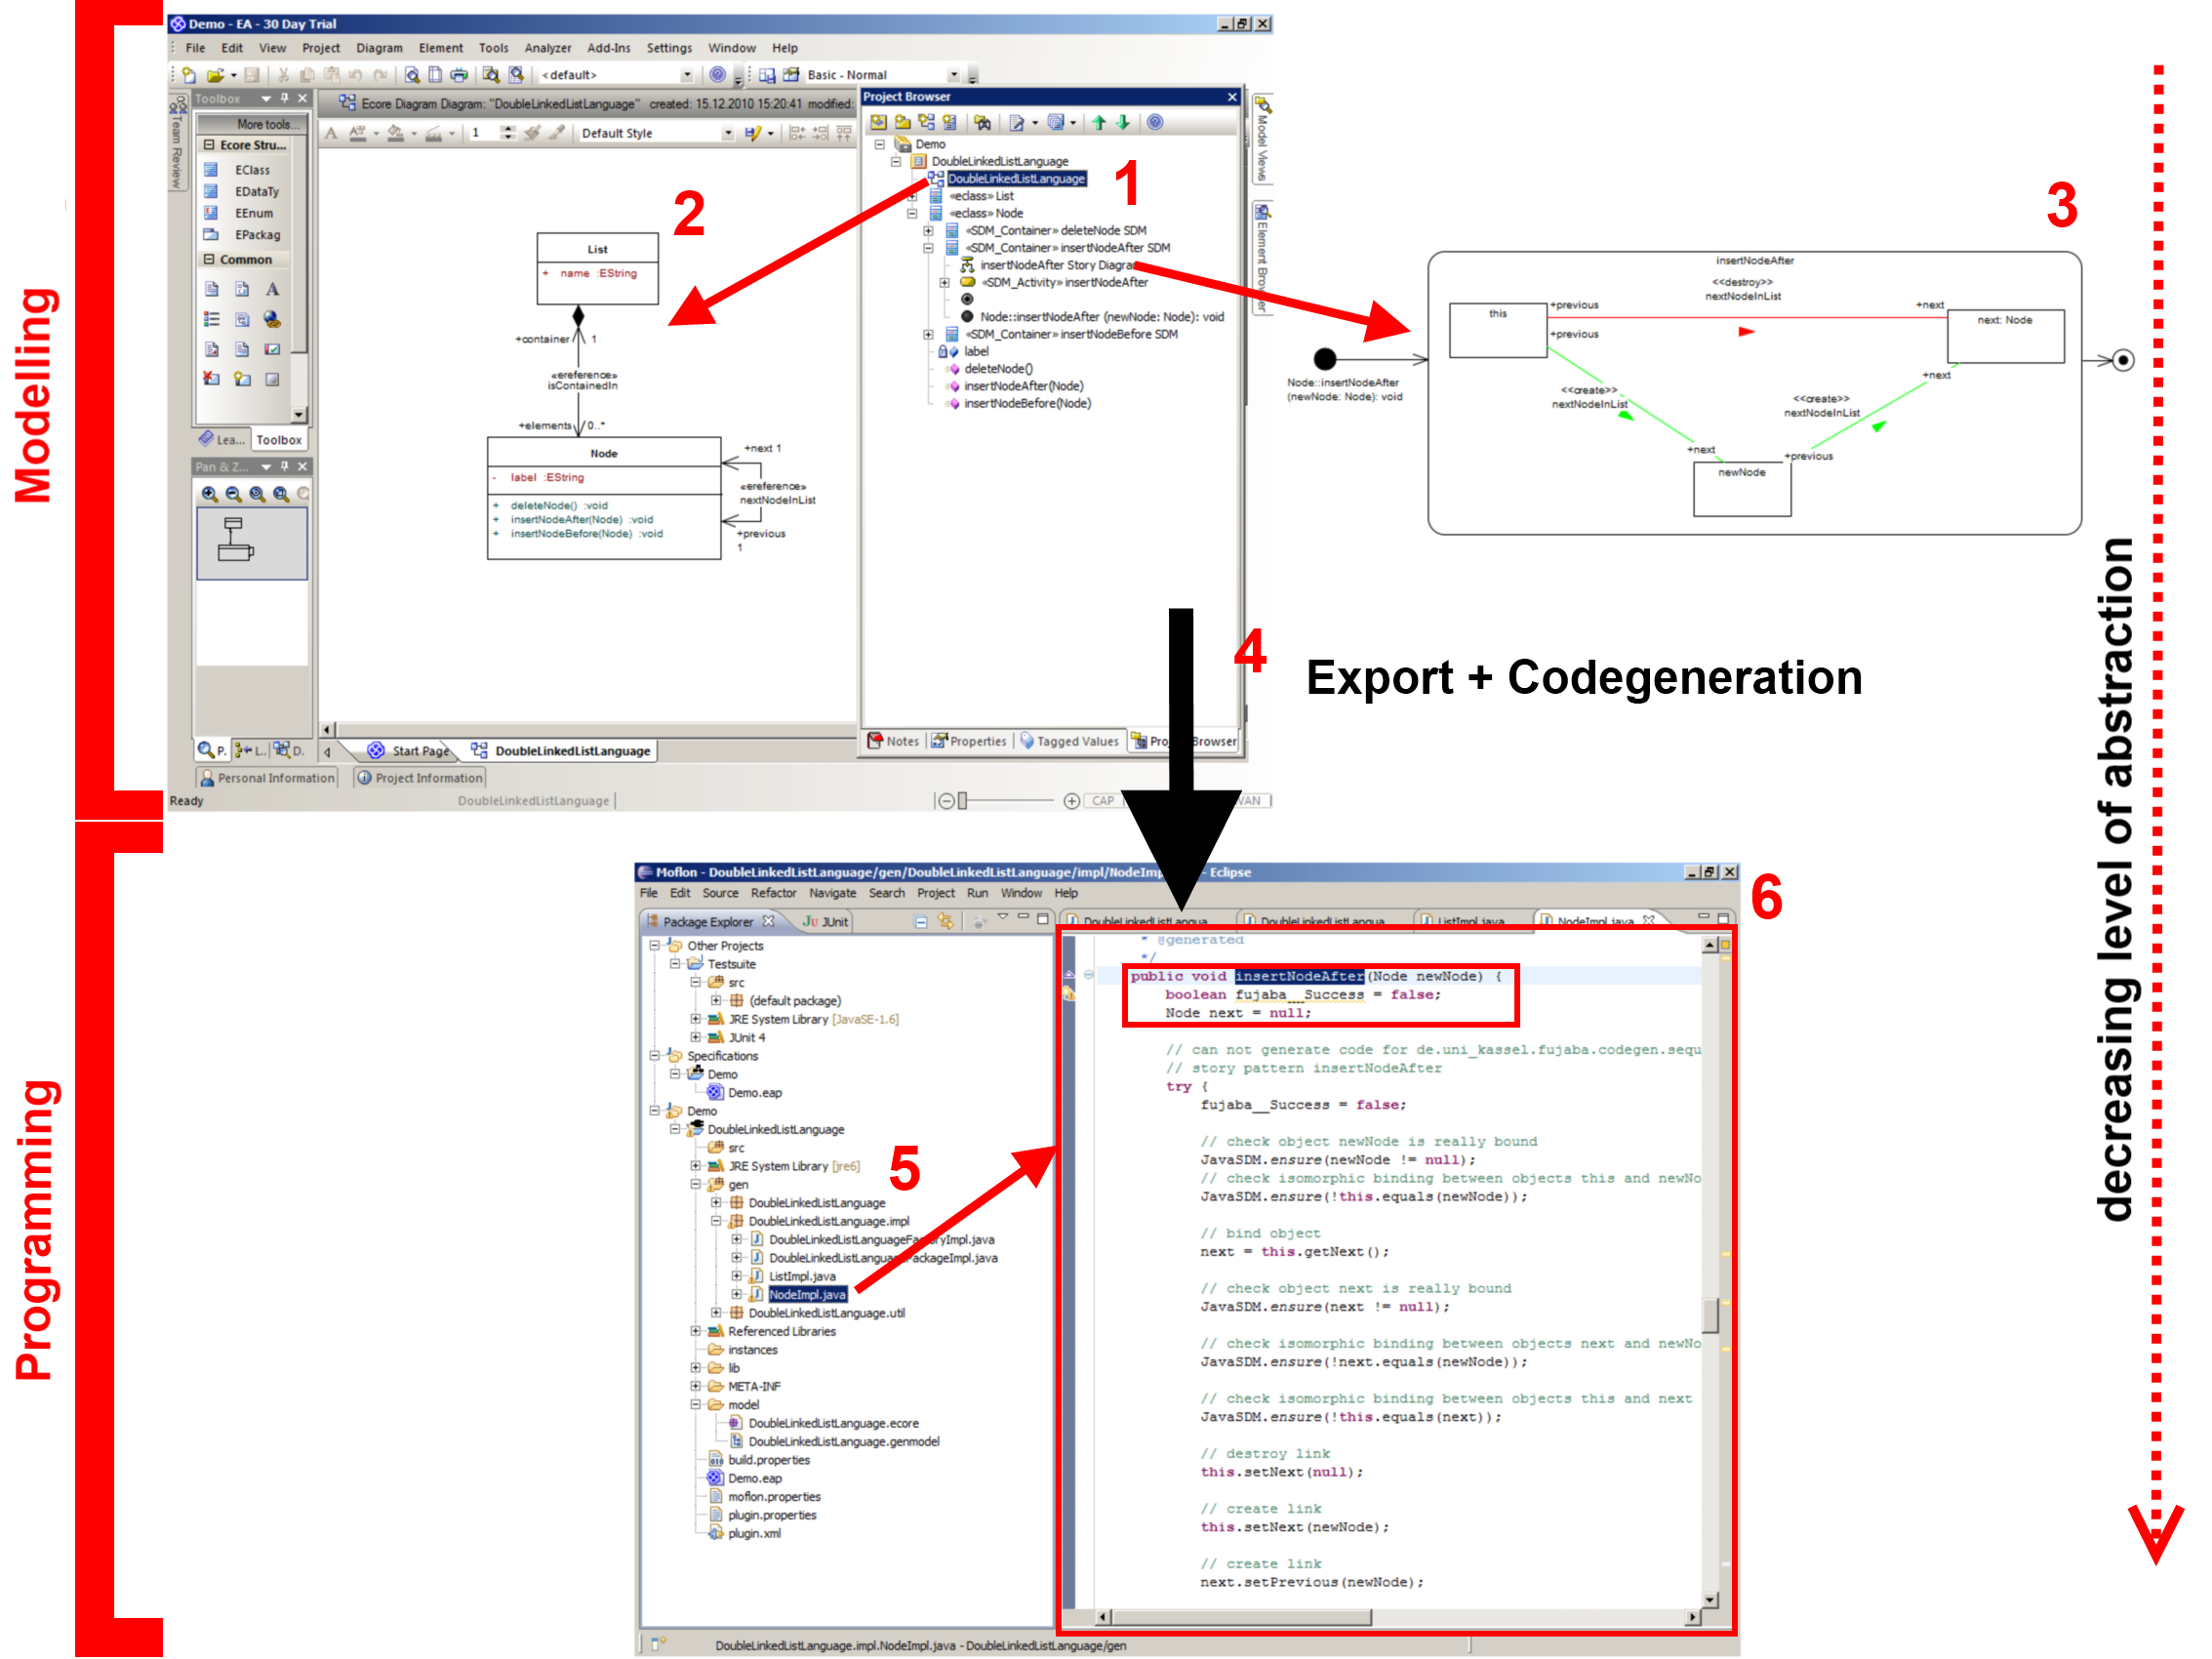
\includegraphics[width=1\textwidth]{tafelbild}
	\caption{Overview}
	\label{fig_Overview}
\end{figure}